\documentclass[a4paper]{article}

\usepackage{fullpage} % Package to use full page
\usepackage{parskip} % Package to tweak paragraph skipping
\usepackage{tikz} % Package for drawing
\usepackage{amsmath}
\usepackage{hyperref}
\usepackage{graphicx}
\usepackage{url}

\title{The Butterfly Effect}
\author{J Campbell}
\date{\today}

\begin{document} % This line start the document

\maketitle

\section{Introduction}
A Non-linear Dynamical System is a sequence of numbers $x_0, x_1, ...$ such that $x_0$ is fixed and $x_{n+1} = \phi(x_n)$ where $\phi$ is some function. When studying Dynamical Systems we are often more interested in general questions than specific results, for example, Does the system eventually settle down?, or, Does the long-term behavior of the system depend on its initial condition?. Even simple Dynamical Systems can yeild interesting results to these questions and in this document we will be looking at one in particular, the Logistic Map.


\section{Logistic Map}
The Logistic Map is defined such that $\phi(x)=\lambda x(1-x)$ where $ 0 <\lambda \leq 4$ and $0\leq x\leq 1$. ie;

$x_{n+1} = \lambda x_n(1-x_n)$, $0 \leq x_n \leq 1 $. I have used sage to plot the Logistic Map in \ref{logisticmap}. The line $y=x$ is included because it clearly illustrates the idea of stationary point.
\begin{figure}[!htbp]
\begin{center}
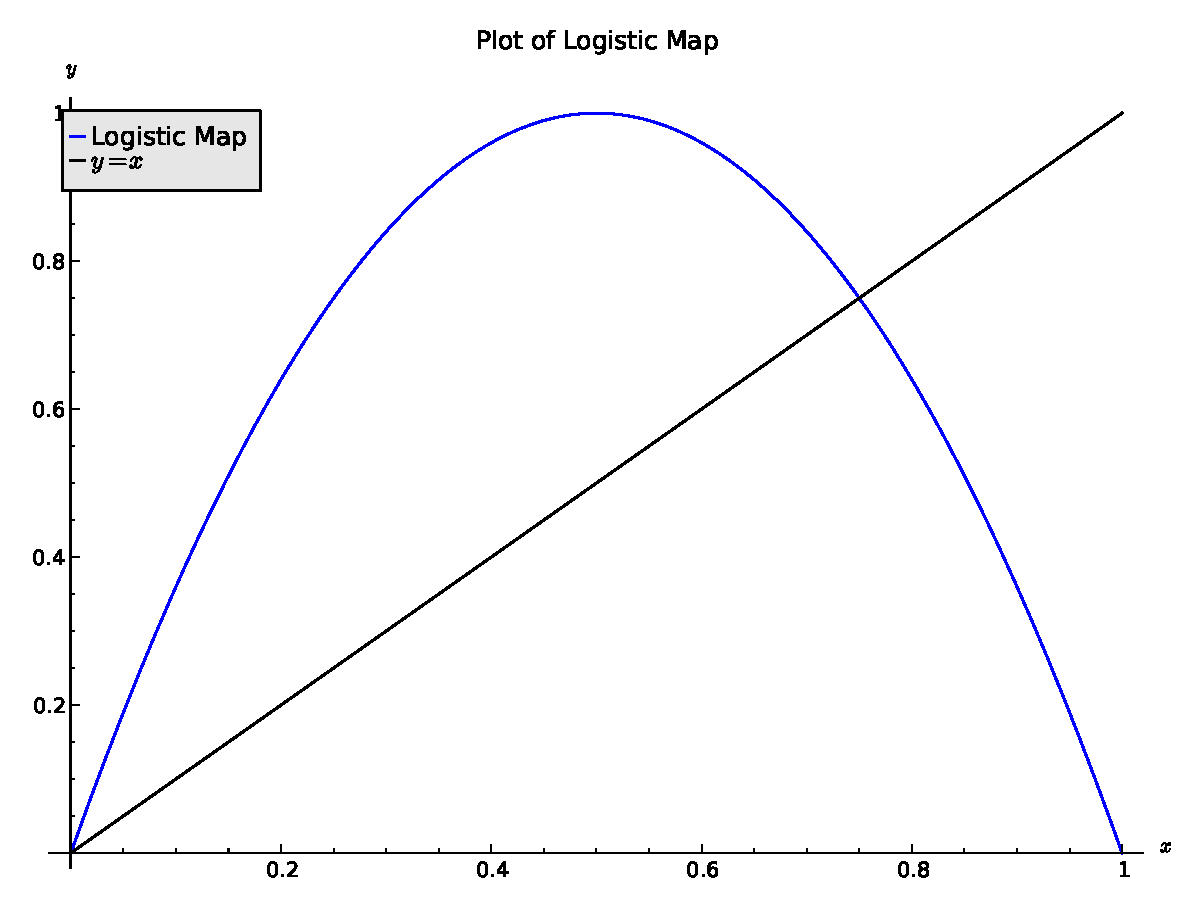
\includegraphics[scale=0.4]{images/logisticmap}
\end{center}
\caption{The Logistic Map where $\lambda = 4$ and the line $y = x$.}
\label{logisticmap}
\end{figure}

\section{Stationary Points}
Stationary Points occure when $x_{n+1}=x_n$. We can find them by solving the equation $\phi(x)=x$. The behaviour of a stationary point can be described as stable or unstable. When a stationary point is stable, other points close to it will be 'attracted', an unstable point has the opposite effect, points diverge away from it. The location of our stationary point is very easy to compute by hand, and gives the solution: $x=3/4$ and $x=0$ when $\lambda =4$. A more interesting question is whether these stationary points are stable.

\begin{verbatim}
logistic(x) = 4*x*(1-x)
solve(logistic(x) == x,x)
\end{verbatim}


\section{The Butterfly Effect}
The Butterfly Effect is a common term used to describe the behaviour of a non-linear dynamical system. The name, coined by Edward Lorenz, is derived from the theoretical example of a hurricane's formation being contingent on whether or not a distant butterfly had flapped its wings several weeks earlier. \cite{wiki:ButterflyEffect} It refers to how the choice of initial starting index can have large impacts later on.
\begin{figure}[htdp]
\begin{center}
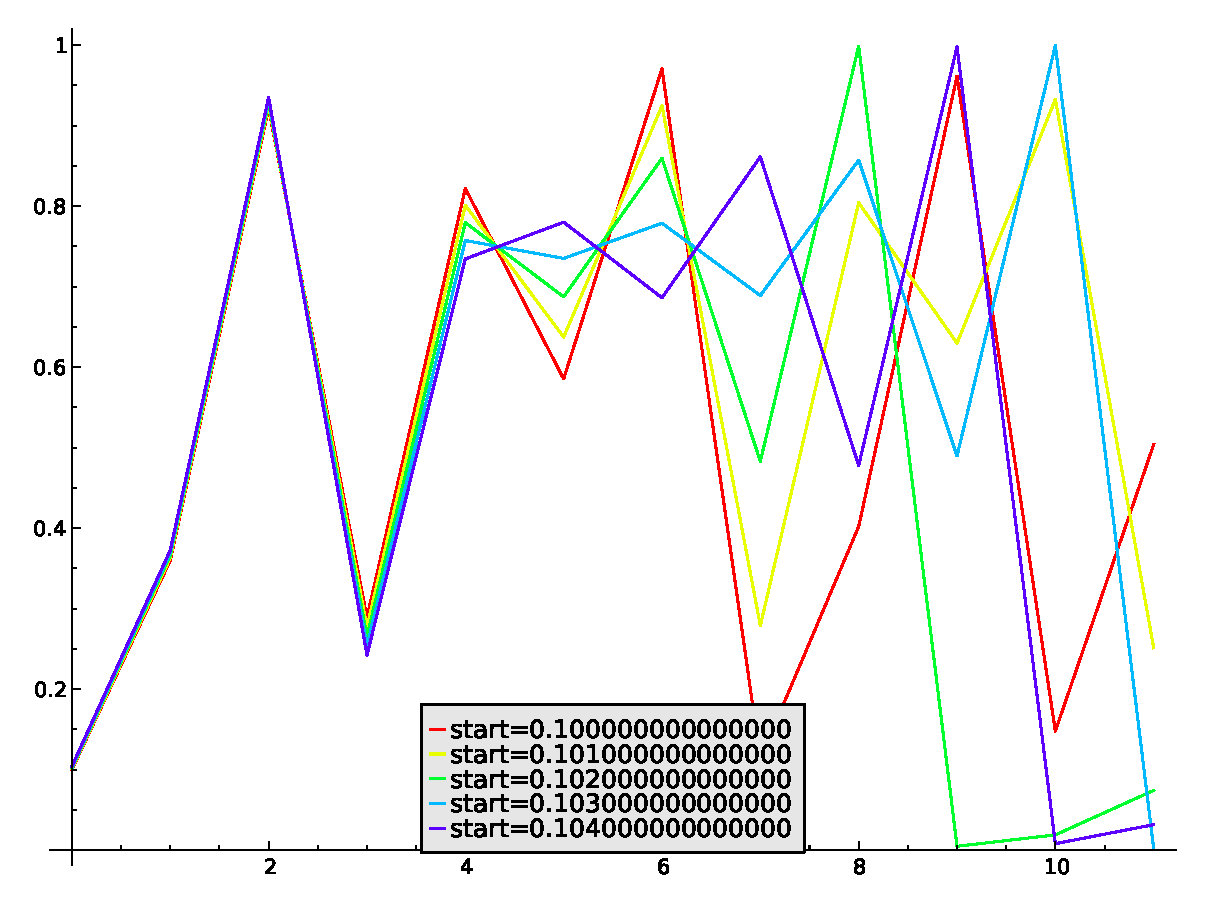
\includegraphics[scale=0.5]{images/butterflyeffect}
\end{center}
\caption{The Logistic Map over 12 iterations using 5 different starting points.}
\label{butterflyeffect}
\end{figure}

\bibliographystyle{plain}
\bibliography{biblio}
\end{document}
%sagemathcloud={"zoom_width":120}